\documentclass[]{final_report}
\usepackage{graphicx}
\usepackage{hyperref}
\usepackage{listings}
\usepackage{graphicx}
\usepackage[backend=bibtex]{biblatex}
\addbibresource{refs.bib}


%%%%%%%%%%%%%%%%%%%%%%
%%% Input project details
\def\studentname{James Arnott}
\def\reportyear{2022}
\def\projecttitle{Comparison of Image Classification Models with Transfer Learning}
\def\supervisorname{Li Zhang}
\def\degree{BSc (Hons) in Computer Science}
\def\fullOrHalfUnit{Full Unit} % indicate if you are doing the project as a Full Unit or Half Unit
\def\finalOrInterim{Interim Report} % indicate if this document is your Final Report or Interim Report

\begin{document}

\maketitle

%%%%%%%%%%%%%%%%%%%%%%
%%% Declaration

\chapter*{Declaration}

This report has been prepared on the basis of my own work. Where other published and unpublished source materials have been used, these have been acknowledged.

\vskip3em

Word Count:

\vskip3em

Student Name: \studentname

\vskip3em

Date of Submission:

\vskip3em

Signature:
\begin{figure}[ht!]
  
\includegraphics[width=50mm]{images/signature.jpg}
\end{figure}

\newpage

%%%%%%%%%%%%%%%%%%%%%%
%%% Table of Contents
\tableofcontents\pdfbookmark[0]{Table of Contents}{toc}\newpage

%%%%%%%%%%%%%%%%%%%%%%
%%% Your Abstract here

\begin{abstract}

  Transfer learning is a common, efficient method for training deep learning models.
  It involves using a pre-trained model to extract features from a dataset,
  and then training a new model on top of the extracted features.
  This report compares a variety of different image classification models with transfer learning,
  and evaluates their performance on a dataset of images of flower species and MRI scans of Alzheimer's patients brains.
% TODO: make sure the abstract is up to date
\end{abstract}
\newpage

%%%%%%%%%%%%%%%%%%%%%%
%%% Project Spec
% TODO: do the project spec, not sure what to put here
% TODO: Time scale? I need to show when I did what
% TODO: Software Engineering, show use of GIT and LaTeX, do uml? Show TDD with jupyter notebooks?
% TODO: Summary of completed work
% TODO: Insert or attach the diary

\chapter*{Project Specification}
\addcontentsline{toc}{chapter}{Project Specification}
Your project specification goes here.

%%%%%%%%%%%%%%%%%%%%%%
%%% Introduction
\chapter{Introduction}

\chapter{Neural Networks}
\begin{figure}[ht!]
  \centering
  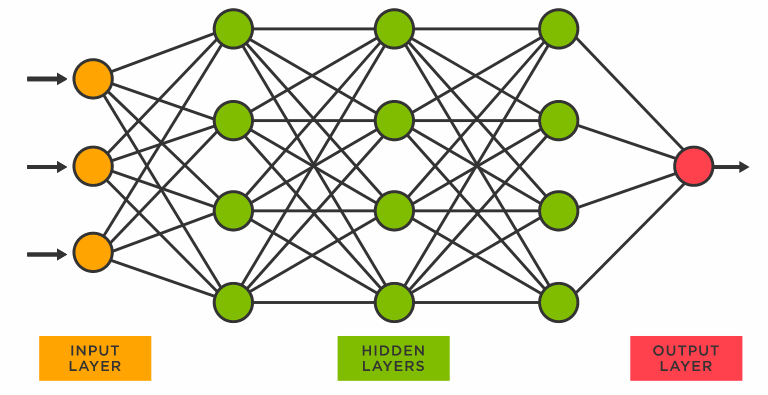
\includegraphics[width=100mm]{images/NeuralNetwork.png}
  \caption{A diagram of a neural network \cite{NeuralNetworkDiagram}}
\end{figure}

\section{What is a Neural Network}
A neural network is a machine learning model that is inspired by the way the human brain works.
It is made up of a series of layers, each layer is made up of a number of neurons.
Each neuron is connected to every neuron in the next layer, and each connection has a weight associated with it.
The weights are used to determine how much each neuron in the next layer is affected by the current neuron.
The weights are updated during training, and the process of updating the weights is known as backpropagation.

\section{Why use a Neural Network}
The use of Neural Networks has increased dramatically in recent years, and they are now used in a variety of different applications.
The reason for this is that they are very good at learning complex patterns in data, and they are able to learn 
these patterns without being explicitly programmed to do so. This saves a lot of time and effort when compared to other machine learning techniques.

They are far more flexible than many of the traditional strategies for image classification, due to the fact they can adapt to new data and are
resilliant to noise in the data or changes such as lighting or rotation.

\pagebreak
\section{What are the alternatives to Neural Networks}

This is not an exhaustive list for image classification, but it is a list of some of the most common alternatives to Neural Networks
that produce the best results.

\subsection{Support Vector Machines}
There are a number of different alternatives to Neural Networks, one common alternative is Support Vector Machines.
Support Vector Machines are a type of supervised machine learning model that can be used for both classification and regression.
They work by finding a hyperplane that separates the data into different classes, and then classifying new data based on which side of the hyperplane it is on.
They are very good at classifying data that is linearly seperable, however they are not very good at classifying data that is not linearly seperable,
and they are also very sensitive to noise in the data.

In one study using SVMs to classify Alzheimer's patients, the researchers managed to get an accuracy of 62.64\% using MRI scans of the brain.
They managed to get between 83\% and 90\% accuracy when using SVMs with clinical parameters, however combining the two methods in this study did not improve the accuracy.\cite{10.3389/fneur.2021.640696}

\subsection{Content Based Image Retrieval}
Content Based Image Retrieval (CBIR) is a type of image retrieval system that uses the actual content of an image as the basis for retrieving similar 
images from a large database. It works by extracting the features from the image and then using those features to compare to other images in the database.
The features are usually based on a combination of color, texture, shape, and other attributes. The system then produces a list of images that are similar 
to the one used for the search query. CBIR systems are particularly useful for searching for images that can't be easily described using traditional keywords.

CBIR can be used to identify images that are not in the database by analyzing the content of the images. 
By extracting features from the image such as color, texture, and shape, CBIR can be used to compare the 
content of the query image with the content of the images in the database. It can then return images that are 
similar in content to the query image even if they are not present in the database. 

For example, if the target image was a blue sky with white clouds, then the algorithm would return 
images that had similar features such as a blue sky and white clouds to the target image.

Although this method of image classification would not seem to be very useful for classifying images of Alzheimer's patients, 
a study was done using this method to classify Alzheimer's patients and they had managed to get an accuracy of 87\% using MRI scans\cite{5972513}

For classifying images of flowers it could also be very useful, as it would allow the user to search for images of a specific flower.
This could help identify flowers by recognizing the different characteristics of each flower, such as the shape of the petals, 
the color of the petals, and the overall structure of the flower.

\section{The different optimizers}

In deep learning, optimisers are algorithms used to adjust the parameters of a model in order to minimise a loss function. 
Optimisers are used to improve the accuracy of a model by reducing the error rate. 
Common optimisers used in deep learning include Stochastic Gradient Descent (SGD),
Adaptive Moment Estimation (Adam), and Root Mean Square Propagation (RMSProp).
There are many different optimizers that can be used to train a model, and the one 
that is used depends on the type of problem that is being solved.

The impact using different optimisers can have is dependent on the type of problem being solved. 
For example, SGD is often used for linear regression problems, while Adam is 
better suited for deep learning problems. 
Additionally, the choice of optimiser can also affect the speed of convergence and the accuracy of the model.

\begin{figure}[h]
  \centering
  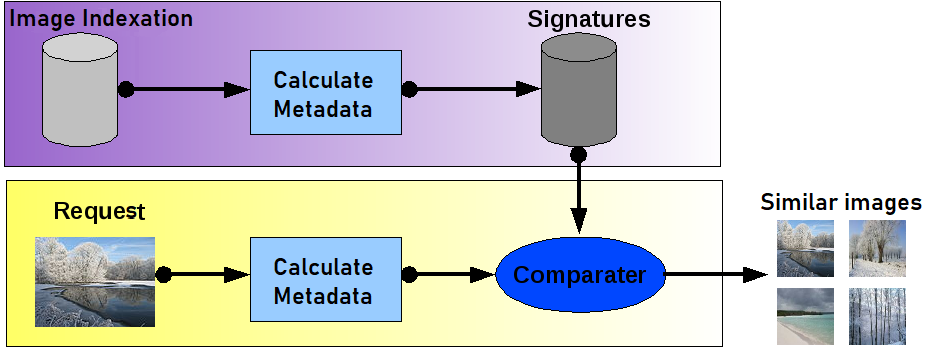
\includegraphics[width=0.7\textwidth]{images/Principe_cbir.png}
  \caption{A diagram of Content Based Image Retrieval \cite{ContentBasedImageRetrieval}}
\end{figure}


\section{What is a Convolutional Neural Network}
A convolutional neural network (CNN) is a type of neural network that is used for image classification.
It is made up of a series of convolutional layers, pooling layers, and fully connected layers.
The convolutional layers are used to extract features from the image, and the pooling layers are used to reduce the size of the image.
The fully connected layers are used to classify the image.
They are often much more efficient than other types of neural networks, and are commonly used for image classification.


\section{Types Of Layers}

% Listing the different types of layers
\begin{itemize}
  \item Convolutional Layer: This layer extracts features from an input image and creates a feature map.

  \item  Pooling Layer: This layer reduces the dimensionality of a feature map while preserving its most important features.
  
  \item  Dropout Layer: This layer randomly ignores nodes during training to reduce overfitting.
  
  \item  Fully Connected Layer: This layer connects all the neurons of the previous layer to every neuron in the next layer. It helps in mapping input to output.
\end{itemize}

% Talk about the different types of layers specifically
% Include a diagram of a CNN


\section{What transfer learning is}
Transfer learning is a common, efficient method for training deep learning models.
There are many different ways to implement transfer learning and here I hope to compare the performance
of a variety of different methods with different pre-trained models.

The applications for transfer learning are vast, and it is a common method for training deep learning models,
This is because it is a very efficient method for training models as most of the work is done by the pre-trained model.
The pre-trained model is used to extract features from the dataset, and then a new model is trained on top of the extracted features.
The pre-trained model is usually frozen so that it does not change during training, and only the new model is trained.

After the new model is trained on top, a process known as fine-tuning can be used to further improve the performance of the model.
Fine-tuning involves training the new model on the dataset, but with a lower learning rate than the initial training.
This is also where the model is usually unfrozen, so that the pre-trained model can be trained as well, which helps to improve the overall performance of the model.

\section{The Models I will be comparing}
The models I have chosen to compare are the MobileNetv3Small\cite{DBLP:journals/corr/abs-1905-02244}, MobileNetv3Large\cite{DBLP:journals/corr/abs-1905-02244}, ResNet50\cite{DBLP:journals/corr/HeZRS15}, ResNet10\cite{DBLP:journals/corr/HeZRS15}, ResNet152\cite{DBLP:journals/corr/HeZRS15}, and InceptionV3\cite{DBLP:journals/corr/SzegedyVISW15} models.
These models are all pre-trained on the ImageNet dataset, which contains 1.2 million images of 1000 different classes.

\section{The Datasets I will be using}
The datasets I have chosen to use for this project are the Oxford 102 Flower Dataset\cite{OxfordFlowers102} and the Alzheimer's MRI Dataset\cite{AlzheimersDataset}.

The choice of datasets is based on the fact that they are both image classification datasets they are both relatively small in classes and
the they have a variety classes ranging in difficulty, which will allow me to compare the capabilities of the different models in a variety of different scenarios.

\chapter{Transfer Learning}

\section{Why use Transfer Learning}
Transfer learning can enable a model to be trained much more efficiently than if it was trained from scratch, as most of the work is done by the pre-trained model.
Aside from the extra time it takes to train a model from scratch, it often requires more training data, which is not always available and can be expensive to obtain.
Transfer learning can often get better results than training a model from scratch, as the pre-trained model has already learned about different features from a large dataset,
and the transfer learning model can then use these features to learn about the new dataset.

\section{Drawbacks of Transfer Learning}
The main drawback of transfer learning is that it is not always possible to use it,
as the pre-trained model may not be able to extract the features from the new dataset.
With image classification, the pre-trained model can typically extract features from any image, but it may not be able to extract the features that are needed for the new dataset.
Transfer learning can also be less efficient than training a model from scratch, 
as the pre-trained model will have all the weights from the original dataset, which may not be needed for the new dataset.
This can cause the model to be less efficient, as it will have to train on weights that are not 
needed but will still affect the performance of the model.

\pagebreak
\section{The code behind the transfer learning}
The code for the transfer learning is shown below.

\begin{lstlisting}[language=Python]
  # This imports the model from the keras library
  MobileNetV3Small = keras.applications.MobileNetV3Small(
    input_shape=(224, 224, 3),
    include_top=False, 
    weights='imagenet')

  # Create the model
  model = keras.Sequential()

  # Freezing all but 10 layers of the pre-trained model
  for layer in MobileNetV3Small.layers[:-10]:
    layer.trainable = False

  # Adding the pre-trained model to the model, along with 
  # a dropout layer and a fully connected layer
  model.add(MobileNetV3Small)
  model.add(keras.layers.Flatten())
  model.add(keras.layers.Dense(512, activation='relu'))
  model.add(keras.layers.Dropout(0.6))
  model.add(keras.layers.Dense(512, activation='relu'))
  model.add(keras.layers.Dropout(0.6))
  model.add(keras.layers.Dense(4, activation='softmax'))
\end{lstlisting}

The code above shows how to create a model using transfer learning,
creating the model structure consists of adding the pre-trained model to the model, 
and then adding a few layers on top of it. The flatten layer is used to flatten the output of the pre-trained model
as that is the input for the fully connected layers. The fully connected layers are used to classify the images.

The dropout layers are used to prevent overfitting, and the dense layers are used to classify the images.
The dense layers are potentially the most important part of the model, as they are the ones that are actually learning about the dataset.
They get trained on the features extracted by the pre-trained model, and the weights of the dense layers are what is used to classify the images.

The final layer of the model is a softmax layer, which is used to classify the images.
It is used to classify the images into one of the classes in the dataset, in this example,
the 4 levels of Alzheimer's disease that are in the Alzheimer's MRI Dataset.

\pagebreak
\section{How to implement Transfer Learning}

\subsection{Extracting features}
Feature extraction is the process of extracting features from the images in the dataset, these features
in the images could be anything, such as the colour, shape, or the texture of the image. All of these features
are used to classify the images, and having these features already extracted can make the training process much faster.
Most of the pre-trained model is usually frozen so that it does not change during the initial stages training, and only the new model is trained,
and on top of the extracted features from the base model.

\subsection{Fine-tuning}
This is the process of training the new model on the dataset, but with a lower learning rate than the initial training and the model is usually unfrozen,
so that the pre-trained model can be trained as well, which helps to improve the overall performance of the model.
This was where I managed to get the best results for my models.

\section{How to fine-tune a model}
Fine-tuning a model is a very simple process, and can be done in just a few lines of code.
The first step is to unfreeze the pre-trained model, which can be done by setting the trainable attribute of the layers to True.
The next step is to set the learning rate to a lower value, which can be done by setting the learning rate attribute of the optimizer.
The final step is to recompile the model, which can be done by calling the compile method of the model.
Here is an example of how I fine-tuned a model using keras:

\begin{lstlisting}[language=Python]
  base_model.trainable = True
  optimizer.learning_rate = 0.0001
  model.compile(optimizer=optimizer, loss=loss, metrics=metrics)
\end{lstlisting}

\begin{verbatim}
  base_model.trainable = True
  optimizer.learning_rate = 0.0001
  model.compile(optimizer=optimizer, loss=loss, metrics=metrics)
\end{verbatim}

\section{The different structures of the models}
There are so many different ways to structure a model and they can 

\section{My training setup}
For this project, I have setup my gaming laptop as a server, with Manjaro\cite{Manjaro} as the operating system.
I've chosen my laptop to do the training on due to it's powerful GPU, which is a NVIDIA GeForce GTX1070\cite{GTX1070}.
This can be used with Nvidia CUDA\cite{CUDA} to speed up the training process, which is what I have done.
Training the models on my laptop has been very useful, as it has allowed me to train the models much easier 
as I can leave it to train overnight without having to constantly check on it.

\chapter{Evaluating the performance}

\section{The different metrics}
% Accuracy
Accuracy is the most common metric used to evaluate the performance of a model, and is defined as the number of correct predictions divided by the total number of predictions.
It is a very simple metric to understand, and is therefore often used to compare the performance of different models.
There is accuracy for both the training and validation sets, and the accuracy of the validation set is used to determine how well the model generalises to new data,
and a validation accuracy that is much lower than the training accuracy is a sign that the model is overfitting.
However, it is not always the best metric to use, as it can be misleading in some cases.

% Loss
Loss is the most common metric used to evaluate the performance of a model, it is calculated by taking the difference between the predicted value and the actual value.
There are however many different types of loss functions, and the one that is used depends on the type of problem that is being solved.
These could be binary cross entropy, categorical cross entropy, or mean squared error. For my project I used binary cross entropy due
to it's simplicity and the fact that it is the most common loss function used for binary classification problems.

% Validation vs Training Loss and Accuracy
The validation loss and accuracy are used to determine how well the model generalises to new data, and a validation loss that is much higher than the training loss is a sign that the model is overfitting.
For the validation set, I have assigned 20\% of the data to be used.

% Confusion Matrix
The confusion matrix is a table that shows the number of correct and incorrect predictions for each class.
It is a very useful metric to use when evaluating the performance of a model, as it can show which classes the model is having the most trouble with.

\section{Data Augmentation}

Data augmentation is the process of artificially increasing the size of a dataset by applying random transformations or filters to the images.
This can help to improve the performance of a model, as it can help to reduce overfitting, and can also help to improve the generalisation of the model.
The transformations that are applied to the images are usually random, and can include things like rotating the image, 
flipping the image, or changing the contrast/saturation of the image.

In the case of the Alzheimer's MRI Dataset, it is extremley useful to have more data to train the model on, as there are a limited number of brain scans available.
MRI scans are also very expensive, so using data augmentation can significantly reduce the cost of training the model.

In the Alzheimer's MRI Dataset, the majority of the archive is comprised of augmented images already however this caused me problems which I will go on to talk about.
With the flower dataset however, I did apply data augmentation to the images, as there were not enough images per class to train the model on.

\section{Problems with the Alzheimer's MRI Dataset and how I fixed them}

\subsection{The problems}
The Alzheimer's MRI dataset that I had chosen early on in the project was far from ideal as I found out later on.
The pre-augmentation that was applied to the dataset caused problems with the training/validation split, as the 
images were already augmented, and the validation set was made up of images that were in the training set, but 
with different transformations applied to them. This gave me amazing results on the validation set, but when I 
tested the model on new data, it performed very poorly. Here the image shows the last 30 epochs of the training process,
and the validation accuracy is very high, higher than what other models from other research papers have achieved.

% Image of the training results
\begin{figure}[h]
  \centering
  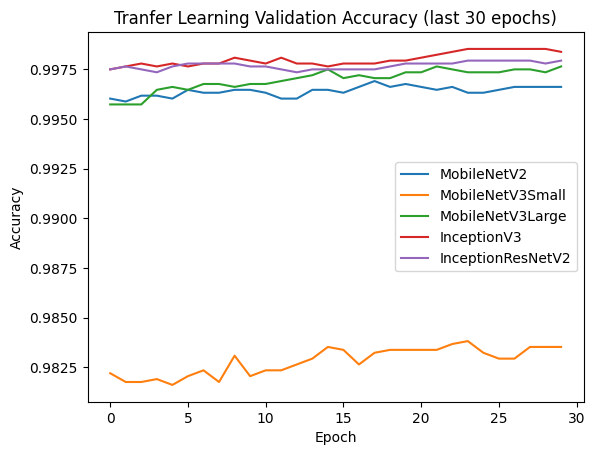
\includegraphics[width=0.7\textwidth]{images/bad-training-result.png}
  \caption{The training results from the various models (Last 30 epochs)}
  \label{fig:training_results}
\end{figure}

\pagebreak

\subsection{The solution}
The solution to this problem was to use the original images, and not the pre-augmented images.
This meant that I had to re-download the dataset, and re-split the dataset into training and validation sets,
and then apply data augmentation to the images. This gave me much better results, and the model was able to generalise
to new data much better. Here is the image of the training results from the various models, and the validation accuracy is much lower than before.

% TODO: Add image of the training results

Here's the snippet of code that I used to augment the images:
\begin{lstlisting}[language=Python]
train_datagen = ImageDataGenerator(rescale=1./255,
    validation_split=0.2,
    featurewise_center=True,
    featurewise_std_normalization=True,
    rotation_range=360,
    width_shift_range=0.1,
    shear_range=0.1,
    zoom_range=0.1,
    height_shift_range=0.1,
    horizontal_flip=True,
    vertical_flip=True,
) # set validation split
\end{lstlisting}

\pagebreak

\section{Evaluating the given metrics}
The metrics of accuracy and loss generally tell us how well the model is performing,
but they do not tell us how well the model is performing for each class.
They do also not tell us how well the model would work in a real world scenario, 
as they are only calculated on the training and validation sets, of which we have a limited amount of data.

The validation dataset is also from the same distribution as the training dataset, 
so it is not a good representation of how well the model would work in a real world scenario 
as the scans could be of a different quality.

I have used the augmented dataset for the training and validation sets as this 
should give a better representation of how well the model would work in a real world scenario.

\begin{figure}[ht!]
  \centering
  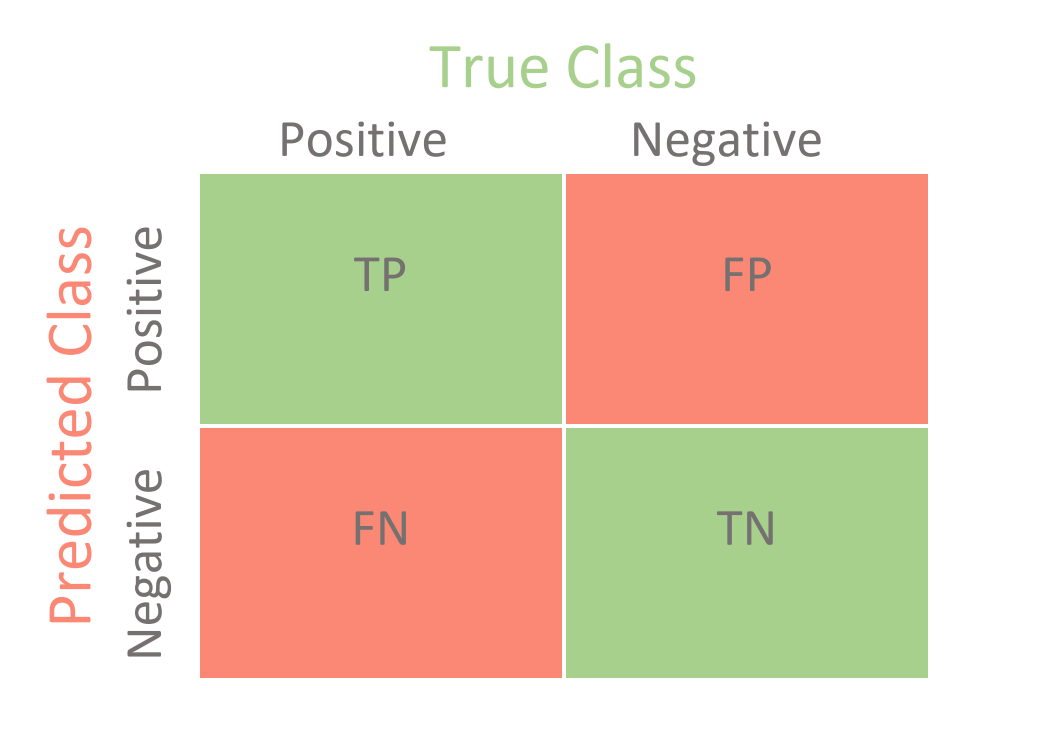
\includegraphics[width=100mm]{images/ConfusionMatrix.png}
  \caption{A confusion Matrix\cite{ConfusionMatrix}}
\end{figure}
\pagebreak
\section{The different datasets}

% images of the datasets
\begin{figure}[ht!]
  \centering
  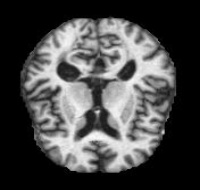
\includegraphics[width=50mm,height=50mm]{images/moderateDemented.jpg}
  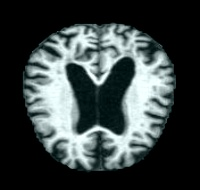
\includegraphics[width=50mm,height=50mm]{images/mildDemented.jpg}
  \caption{The Alzheimer's MRI Dataset\cite{AlzheimersDataset}}
\end{figure}

The Alzheimer's MRI Dataset is a dataset that contains 4 different levels of Alzheimer's disease,
it contains 33984 images in the augmentation folder and the images are all 256x256 pixels in size.
They require resizing to 224x224 pixels in order to be used with the pre-trained models as they are expecting images of that size.
Not using all the resolution of the images is a problem as it could reduce the accuracy of the model,
however it is a nessasary due to the models being trained on images of that size.
It does however not seem to have a significant impact on the accuracy of the model, as I am still able to get a validation accuracy of 99.8\%.
I could in the future potentially crop the black borders of the scans to increase the amount of useful data that is being passed to the model.

\begin{figure}[ht!]
  \centering
  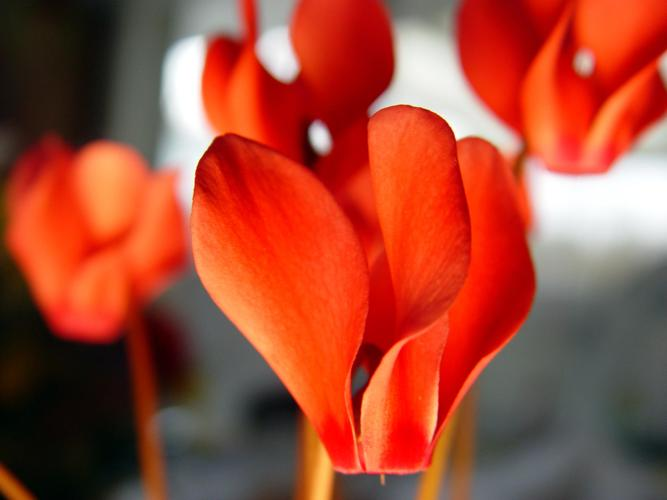
\includegraphics[width=50mm,height=50mm]{images/flower1.jpg}
  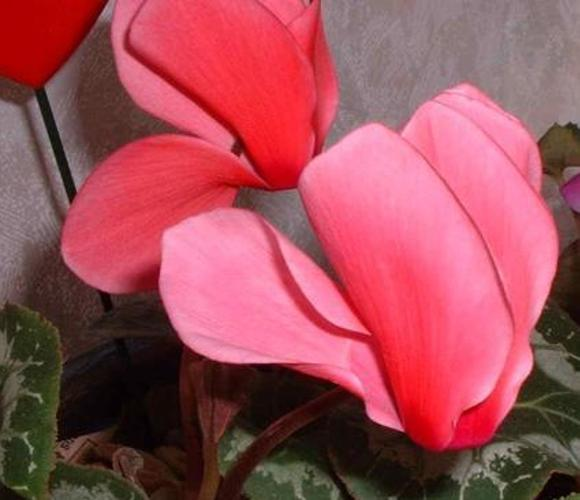
\includegraphics[width=50mm,height=50mm]{images/flower2.jpg}
  \caption{The Oxford 102 Flower Dataset\cite{OxfordFlowers102}}
\end{figure}

The Oxford 102 Flower Dataset is a dataset that contains 102 different types of flowers,
the images are all different sizes, with 3 channels for colour and are in the JPG format.
I have chosen this dataset as it contains a wide variety of images with different backgrounds and lighting conditions,
which should help to test the generalisation of the model, along with the ability for the base model to extract features from the images.
Per class, there are fewer examples than in the Alzheimer's MRI Dataset, however there are still enough to train the model on.
This will be a good test for the various base models to see which one is the best at extracting features from the images.

\chapter{The different models that are being compared}
% TODO: finish
\section{Mobilenetv3}

As described in the "Searching for Mobilenetv3" paper\cite{DBLP:journals/corr/abs-1905-02244}, this model is designed for mobile devices, and is a successor to the Mobilenetv2 model.
It is a comparatively small model as it is optimised for mobile devices, and is also very fast.

The resulting models from this paper are:
\begin{itemize}
    \item Mobilenetv3-Large
    \item Mobilenetv3-Small
\end{itemize}

The idea to have a large and small model is to specialise the model for different use cases and different hardware, increasing the speed or accuracy of the model.
The large model is designed for high accuracy, and the small model is designed for high speed, there may also be cases where the smaller model is the only viable option due to hardware constraints.

% TODO: Talk about Hardware aware network architecture search \cite{DBLP:journals/corr/abs-2101-09336}



\section{Resnet50}

\chapter{Software Engineering}
\section{The code}
The way I have structured the code is by having a main.py file that contains the code to train the model, and a Main.ipynb file that contains the code to test setting up the model.

\section{My Development Environment}
I have used the following tools to develop this project:
\begin{itemize}
    \item Python 3.8.5\cite{Python} - To run the code
    \item Jupyter Notebook\cite{Jupyter} - To help me develop the code and generate the graphs
    \item Visual Studio Code\cite{VsCode} - As my IDE to develop in, I have used the SSH feature of VsCode to SSH into my linux server and modify the code there quickly
    \item GitLab\cite{RHULGitLab} - To store the code and to track the changes
    \item tmux\cite{tmux} - To run the code in the background
    \item CUDA\cite{CUDA} - To train the models on the GPU
\end{itemize}

\section{Using Git}
I have used Git to manage the code, and have used the RHUL GitLab server to host the code.
This was not the first time I have used Git, however it was the first time I have used it with GitLab.
I used seperate branches for the different stages of the project, and then merged them into the master branch when they were complete.
The branches were made to create the different planning papers, and then to setup the development environment.
I also used branches to create the different models, and then to test them too.

All of my commits were in the format of Commitlint\cite{CommitLint} to make it easier to read the commit messages, make them more consistent, 
and to make it easier to go through the history and find a specific change or commit to cherrypick or revert.

\section{Testing with Jupyter Notebook}
I have used Jupyter Notebook to test the code, and to generate the graphs.
This was the most useful tool for me as it allowed me to test the code quickly and easily,
I had many issues with setting up the code as this was the first time I have trained any model.

\section{Using tmux}
I have used tmux to run the code in the background, this was useful as I could SSH into my server and run the code, and then disconnect from the server.
I would then periodically SSH back into the server to check on the progress of the code, and to see if there were any errors.
This wasn't ideal as I could have setup a canary to send me an email if there were any errors, however I didn't have time to do this.

\section{Using Test Driven Development}
The tests I wrote for my code were esentially just the graphs that I generated, as I was testing the code by generating the graphs
and then checking that the graphs were looking correct. This was really the only way I could test the code, as the models take 10+ hours to train,
and I didn't have the time to train the models multiple times to see if unit tests that I had written were correct.

In the future I would like to use unit tests as I could setup an automated pipeline to train the models and then run the unit tests,
and then if the unit tests fail, then the pipeline would fail and I would be notified. This would allow me to test the code more easily,
and to make sure that the code is working correctly. I would also be able to test the code on a smaller dataset, which would allow me to train the models quicker,
and to test the code quicker.

Aside from testing the models, I could setup unit tests for an API that I could create for anyone to upload their brain scans to and get a prediction of whether they have Alzheimer's or not.
This would give me an oppourtunity to write unit tests for the API, and to test the code that I would write for the API.


\chapter{Optimising the training}
% talk about the different optimizers and how they affect the performance of the models

\section{Different learning rates}

When training a model, the learning rate is the rate at which the model learns from the data.
A low learning rate will cause the model to learn slower, and a high learning rate will cause the model to learn quicker
but it can also cause the model to get stuck in a local minimum. A combination of a high learning rate whilst the base model is frozen,
and a low learning rate whilst the base model is unfrozen is a good way to train a model as it allows the model to learn quickly at the start,
and then fine-tune the model at a slower rate. 

% Also talk about the different learning rates and how they affect the performance of the models

\section{Batch sizes}

The batch size is the number of images that are passed to the model at a time.
A larger batch size will cause the model to learn quicker, however it will also use more memory whereas
having a smaller batch size will cause the model to learn slower, however it will use less memory.
When I started off, I did not understand the concept of batch sizes, and I was using a batch size of 1000, this lead to my training times
being very long and I had to wait days for a model to train.
I have found that a batch size of 32 works well for the models that I have trained and my GTX1070 8GB GPU\cite{GTX1070} doesn't often run out of memory.

\section{Dataset Augmentation}

When training a deep learning model, it is important to have a large dataset, as this will allow the model to learn from a wide variety of data.
Unfortunatly I do not have as many MRI scans as I would like, so I have used data augmentation to increase the size of the dataset.
Using the ImageDataGenerator class from Keras\cite{Keras}, I have been able to generate new the new images.
This helps training the model as it allows the model to learn from a wider variety of data, and it also helps to prevent overfitting.
It is not optimal to be required to use data augmentation, however it's significantly better than not having enough data to train the model.
If these models were to be used in a real world scenario, augmentation helps to make the model more resiliant to the quality of the scans.

\chapter{My training results}
% TODO: add graphs and talk about the results
\subsection{The comparison of the different models}
Here is a graph of all the different models that I have trained properly with the Alzheimer's dataset.
The graph shows the accuracy of the models on the validation set along with the accuracy on the training set.
\begin{figure}[h]
  \centering
  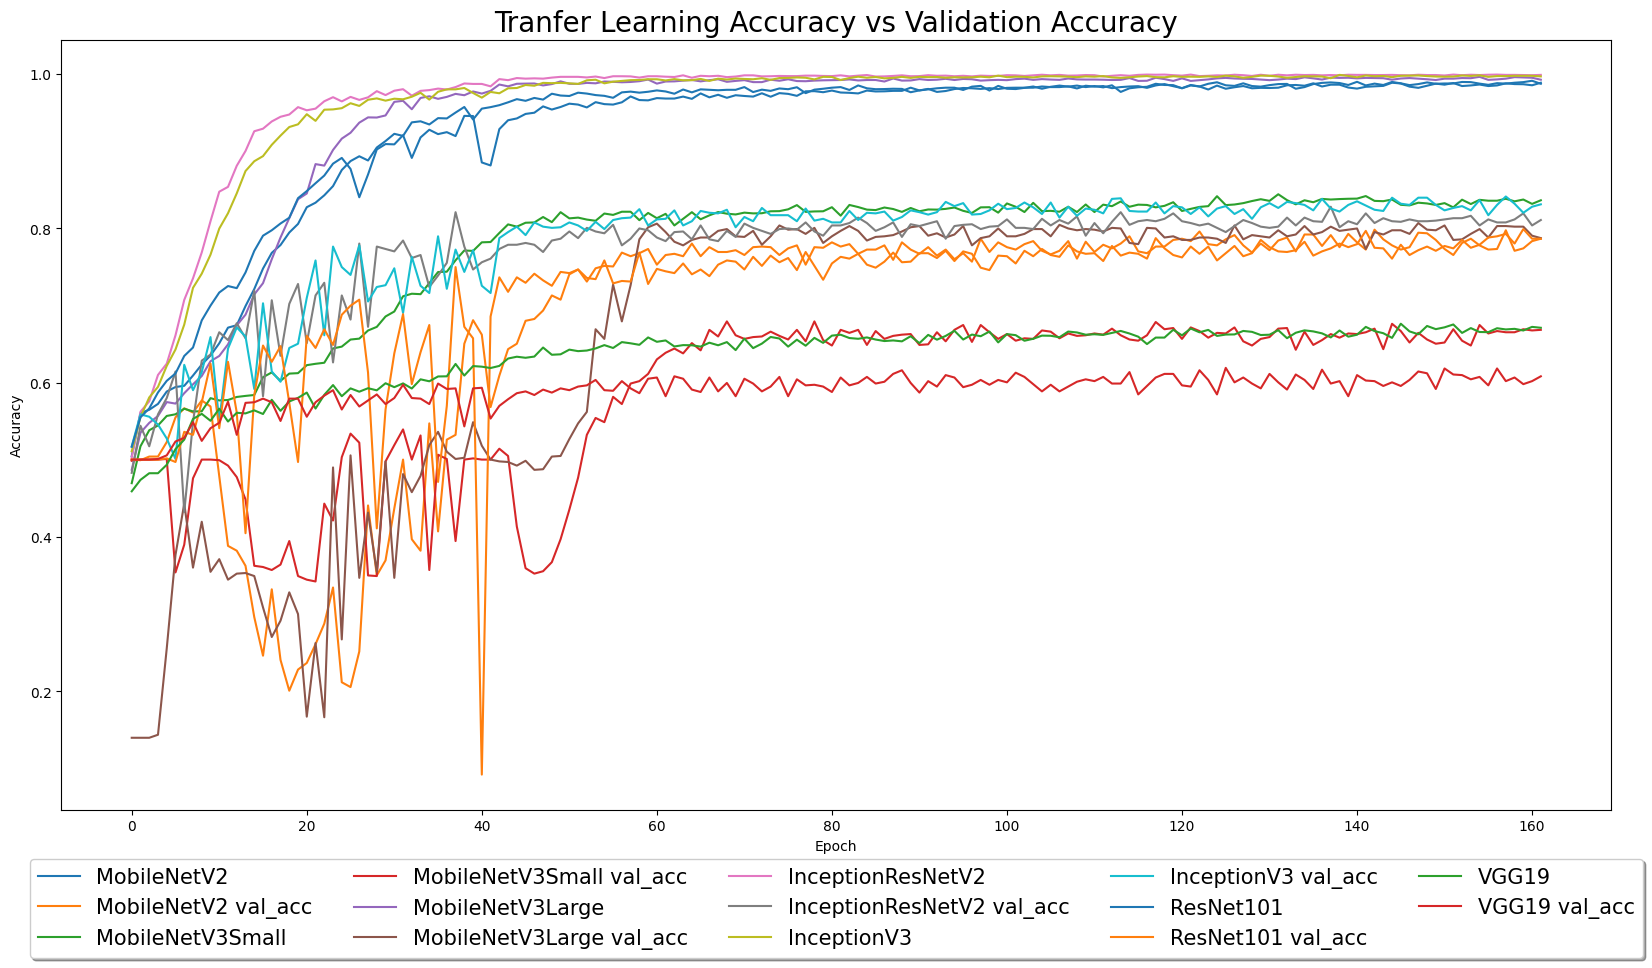
\includegraphics[width=1\textwidth]{images/good-training-acc-vs-val.png}
  \caption{The accuracy of the different models}
  \label{fig:loss}
\end{figure}
\pagebreak
\subsection{InceptionV3}
For my training results, when everything was working correctly, I was able to get a highest validation accuracy of 84\% and a loss lowest of 0.30.
% Show the graphs of the training results
\begin{figure}[ht!]
  \centering
  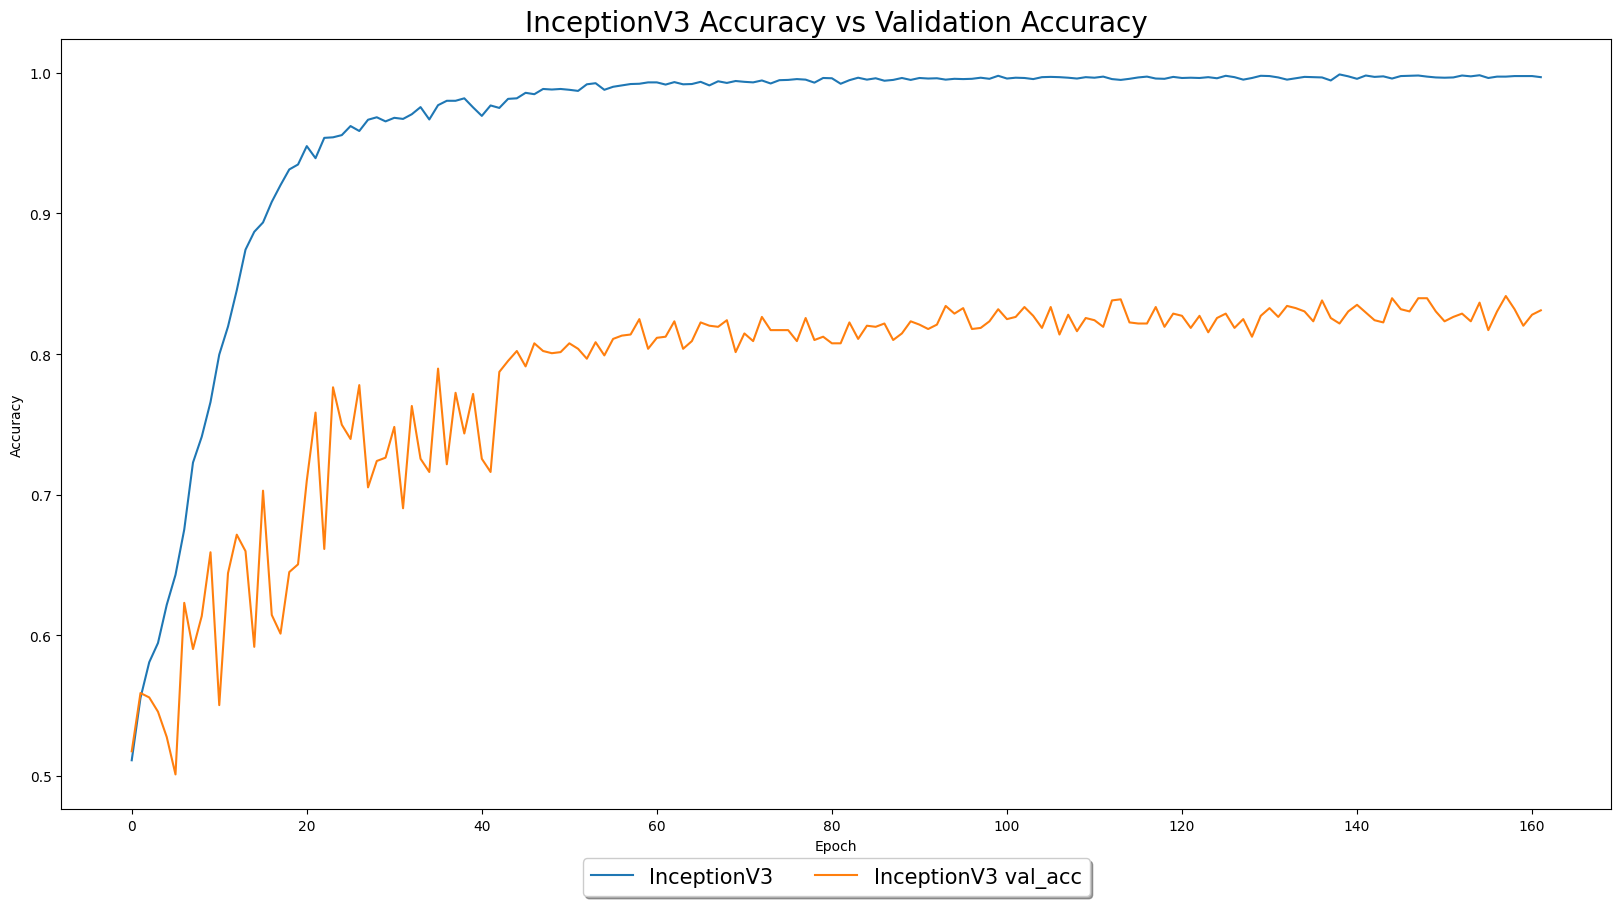
\includegraphics[width=120mm]{images/inceptionv3-accuracy-vs-val-acc.png}
  \caption{The training results using InceptionV3\cite{DBLP:journals/corr/SzegedyVISW15} as the base model}
\end{figure}

This graph clearly indicates that there was overfitting, as the validation accuracy is significantly lower than the training accuracy.
This is due to the fact that the model is learning from the training data, and it is not generalising well to the validation data.
To help mitigate overfitting, I did use data augmentation and dropout layers, however I think that the base model it's self is overfitting to the data.

I will need to do more research into regularisation techniques to help mitigate overfitting, and to help improve the performance of the model.
To avoid this in the future, I will use more advanced techniques such as hyperparameter tuning and regularisation.

L2 and L1 regularisation techniques work by adding a penalty to the weights of the model, which helps to reduce overfitting.
Hyperparameter tuning is a process of optimising the hyperparameters of a model, such as learning rate, number of layers, etc. 
This helps to improve the accuracy of the model and reduce overfitting.
\pagebreak
\subsection{The model sizes}

Here's a barchart comparing the sizes of the models in megabytes. 
They are uncompressed and include the full model, after transfer learning.

\begin{figure}[ht!]
  \centering
  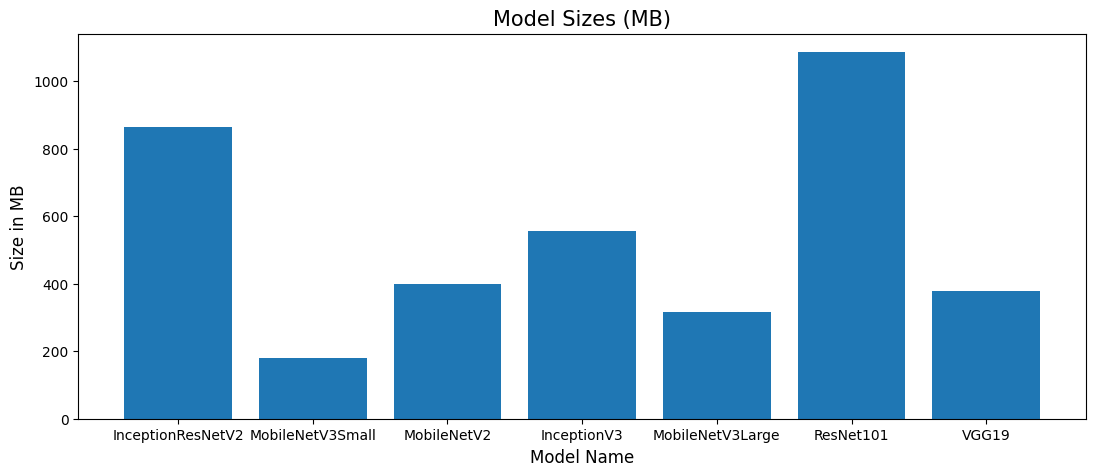
\includegraphics[width=120mm]{images/model-sizes.png}
  \caption{The different model sizes in MB}
\end{figure}

From this graph, it's clear to see how large some of the models are in comparison to each other.
The largest model, ResNet101 is just over 1GB in size and has a far worse accuracy than the top performing model, InceptionV3.

\begin{figure}[ht!]
  \centering
  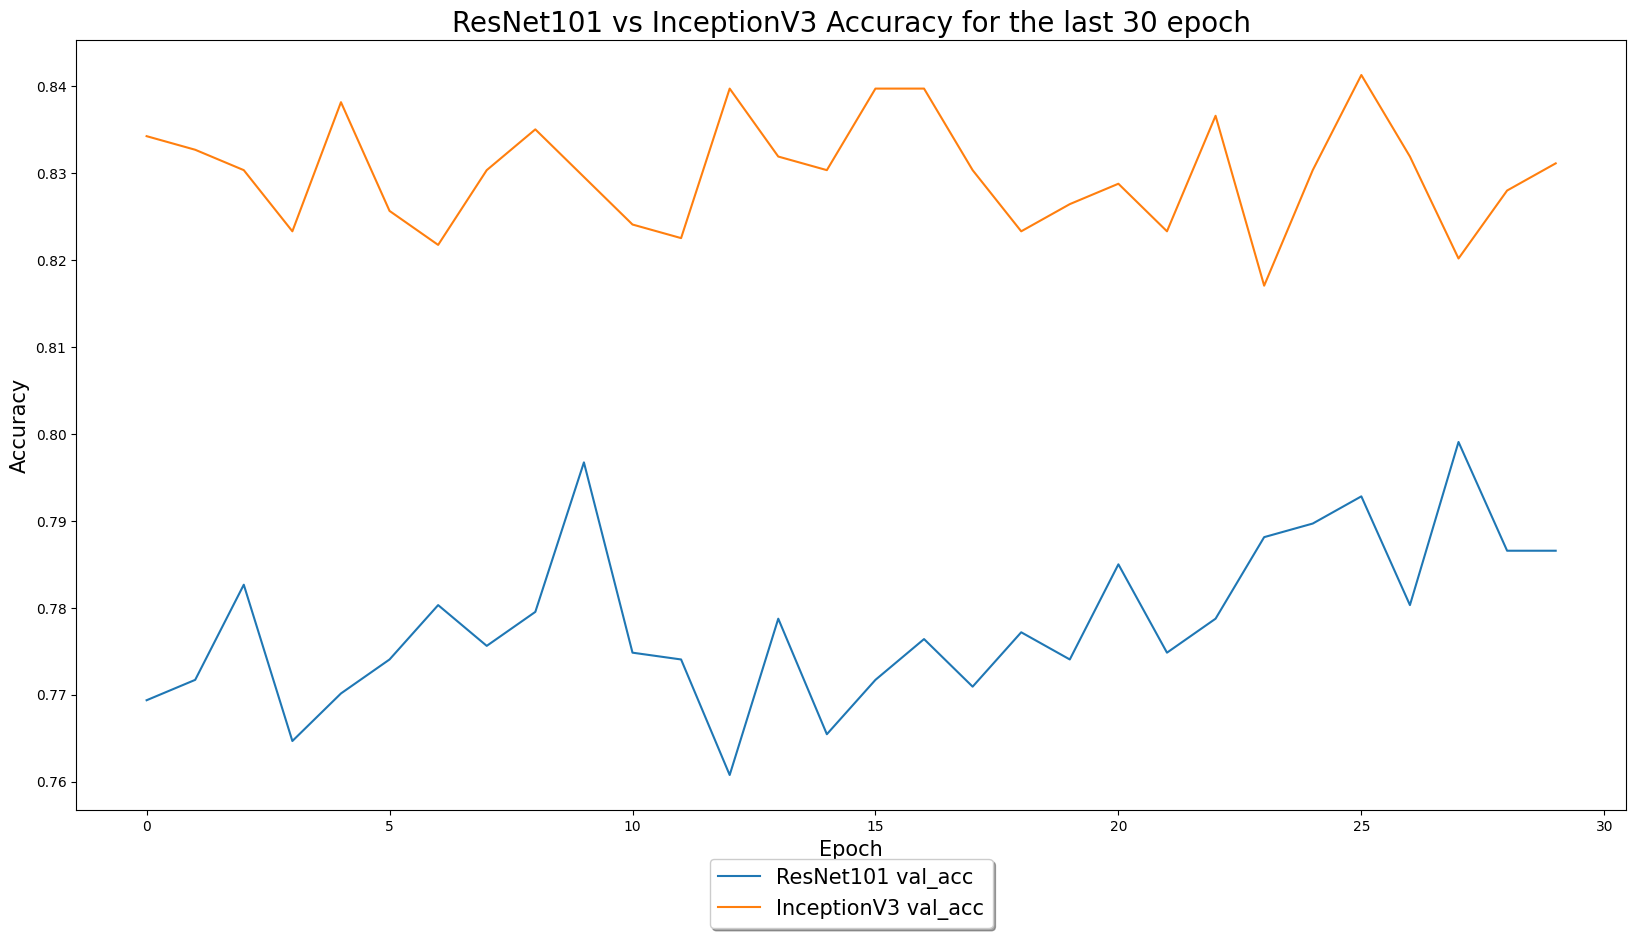
\includegraphics[width=120mm]{images/ResNet101-vs-Inceptionv3.png}
  \caption{Here's it's performance in comparison to InceptionV3}
\end{figure}

The ResNet101\cite{DBLP:journals/corr/HeZRS15} model was created by Microsoft and is a 101 layer deep neural network.
It was created to compete in the ImageNet Large Scale Visual Recognition Challenge\cite{ILSVRC} in 2015.
Inceptionv3 is a 48 layer deep neural network, and was created by Google to compete in the same challenge in 2015.

Although the ResNet model managed to win the challenge, it is clear to see that Inceptionv3 is a far better model for this problem.
Both models were trained on the same dataset (ImageNet), however the imagenet dataset is very different to the Alzheimer's dataset.
The imagenet dataset contains a wide variety of images, whereas the Alzheimer's dataset contains a very small number of images and they are all MRI scans, with only 4 classes.
This could suggest that the ResNet model performs better on a larger dataset, however it is not as good at classification with a smaller dataset and fewer classes.

\chapter{Conclusion}

This project is a great learning experience for me, and I have learned a lot about transfer learning and how to implement it.
Before I started this project, I had never used transfer learning before, and had only used pre-trained machine learning models for image classification.
I have learned a lot about the different types of models, how they are structured, and how they can be used for transfer learning.

\section{What I have learned}
I have specifically learnt how complex image classification models are structured, as they are far more complex than I had initially thought.
% talk about mobilenetv3

\section{What I will do differently}
I need to spend more time researching the different structures of the models, and how the optimal ways they can be used for transfer learning.
This would help with optimising what layers should be frozen and which should be unfrozen at different stages of the training process.

\section{What I need to do next}



\newpage
\printbibliography
\label{endpage}
\end{document}
\end{article}